\documentclass[tikz,border=8pt]{standalone}
% Shared look for every TikZ diagram. Load with \input{../../tools/tikz-style.tex}
\usepackage[T1]{fontenc}
\usepackage{lmodern}
\renewcommand{\sfdefault}{lmr}  % diagrams use the same serif as the text
\usetikzlibrary{arrows.meta, positioning, shapes.geometric, calc, fit, backgrounds}
\definecolor{cblue}{HTML}{4C78A8}
\definecolor{corange}{HTML}{F58518}
\definecolor{cgreen}{HTML}{54A24B}
\definecolor{cred}{HTML}{E45756}
\definecolor{cpurple}{HTML}{B279A2}
\definecolor{cgrey}{HTML}{6B6B6B}
\tikzset{
  every picture/.style={font=\sffamily, line width=1.2pt},
  box/.style={draw=#1, fill=#1!12, rounded corners=4pt, align=center, inner sep=7pt, minimum height=1.1cm},
  box/.default=cgrey,
  arrow/.style={-{Stealth[length=3mm]}, draw=cgrey, line width=1.4pt},
  title/.style={font=\sffamily\bfseries\Large},
  note/.style={font=\sffamily\small, text=cgrey, align=center},
}
\AtBeginDocument{\hyphenpenalty=10000 \exhyphenpenalty=10000}

\begin{document}
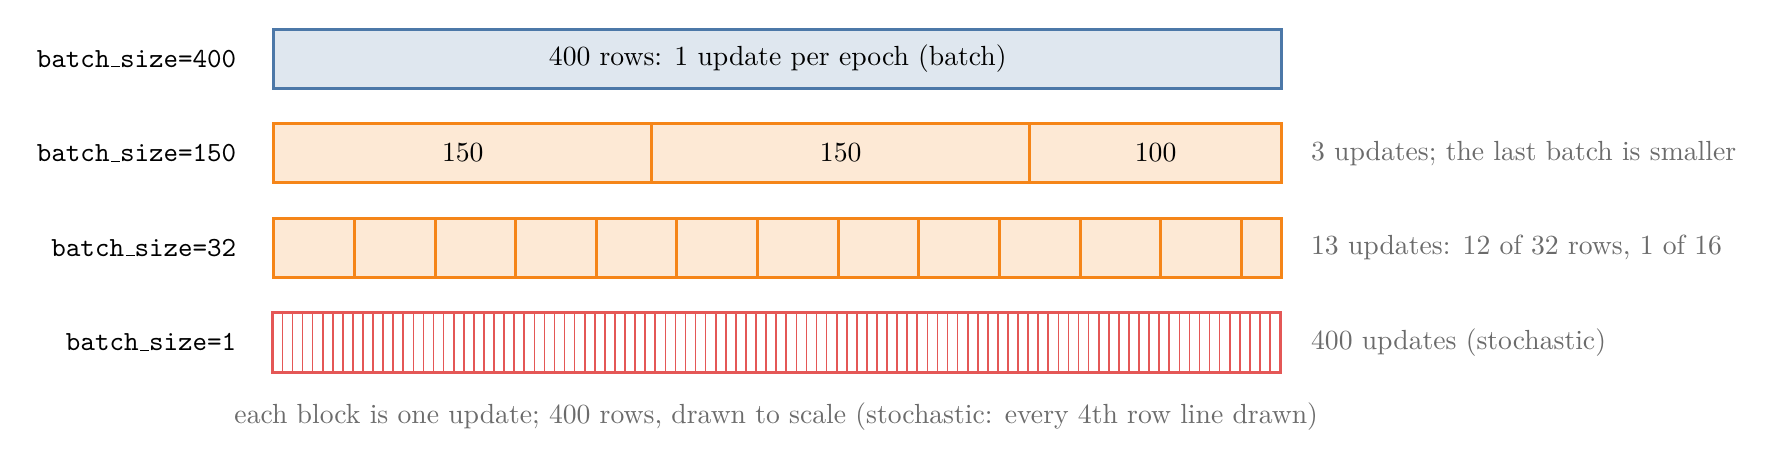
\begin{tikzpicture}[x=0.032cm,
  b/.style={draw=#1, fill=#1!18, line width=1.1pt, minimum height=0.75cm, inner sep=0pt, font=\sffamily}]
  % each row: label, then the batches of 400 rows drawn to scale
  \node[anchor=east, font=\sffamily] at (-10, 0) {\texttt{batch\_size=400}};
  \node[b=cblue, minimum width=12.8cm, anchor=west] at (0, 0) {400 rows: 1 update per epoch (batch)};
  \node[anchor=east, font=\sffamily] at (-10, -1.2) {\texttt{batch\_size=150}};
  \node[b=corange, minimum width=4.8cm, anchor=west] at (0, -1.2) {150};
  \node[b=corange, minimum width=4.8cm, anchor=west] at (150, -1.2) {150};
  \node[b=corange, minimum width=3.2cm, anchor=west] at (300, -1.2) {100};
  \node[anchor=west, note, font=\sffamily\normalsize] at (408, -1.2) {3 updates; the last batch is smaller};
  \node[anchor=east, font=\sffamily] at (-10, -2.4) {\texttt{batch\_size=32}};
  \foreach \i in {0,...,11} \node[b=corange, minimum width=1.024cm, anchor=west] at (32*\i, -2.4) {};
  \node[b=corange, minimum width=0.512cm, anchor=west] at (384, -2.4) {};
  \node[anchor=west, note, font=\sffamily\normalsize] at (408, -2.4) {13 updates: 12 of 32 rows, 1 of 16};
  \node[anchor=east, font=\sffamily] at (-10, -3.6) {\texttt{batch\_size=1}};
  \foreach \i in {0,4,...,396} \draw[cred, line width=0.6pt] (\i, -3.98) -- (\i, -3.22);
  \draw[cred, line width=1.1pt] (0, -3.98) rectangle (400, -3.22);
  \node[anchor=west, note, font=\sffamily\normalsize] at (408, -3.6) {400 updates (stochastic)};
  \node[note, font=\sffamily\normalsize] at (200, -4.55) {each block is one update; 400 rows, drawn to scale (stochastic: every 4th row line drawn)};
\end{tikzpicture}
\end{document}
